\documentclass[a4paper]{article}
\let\subsubsubsection\paragraph
\let\subsubsubsubsection\subparagraph
\setcounter{secnumdepth}{4}
\setcounter{tocdepth}{4}
\usepackage[utf8]{inputenc}
\usepackage[T1]{fontenc}
\usepackage[italian]{babel}
\usepackage{graphicx}
\usepackage{lscape}
\usepackage{fancyhdr}
\usepackage{totpages}
\usepackage{enumerate}
\usepackage{float}
\usepackage{color}
\usepackage[pdftex]{hyperref}
\usepackage{listings}
\usepackage{tabularx}
\usepackage{amsthm}
\hypersetup{colorlinks,breaklinks,linkcolor=blue,urlcolor=black}

\usepackage{fancyhdr}
\newcommand{\fncyblank}{\fancyhf{}}
%\newenvironment{abstract}%
%{\fncyblank\null\vfill\begin{center}%
%\bfseries\abstractname\end{center}}%
%{\vfill\null}

\renewcommand{\baselinestretch}{1.25}

\pagestyle{fancy} 

\makeindex

% Definizione di nuovi "tokens" (e valori che possono assumere)
\newtoks\titolo
\newtoks\sottotitolo
\newtoks\filename
\newtoks\data
\newtoks\versione
\newtoks\distribuzione

% Titolo documento + titolo a pie' pagina e data (tokens)
\titolo={F1 Simulator} 
\sottotitolo={Progetto di Sistemi concorrenti e distribuiti} 
\data={16 Ottobre 2010}

% Informazioni documento (tokens)
\filename={Relazione.pdf}
\versione={1.2}
\distribuzione={Prof. Vardanega Tullio \\
		     	& Miotto Nicola \\
			& Nesello Lorenzo
}

% Header (left, center, right)
\lhead{} 
\chead{}
\rhead{}
\renewcommand{\headrulewidth}{0.4pt}
% Footer (left, center, right)
\lfoot{} \cfoot{} \rfoot{\thepage/\pageref{TotPages}}
\renewcommand{\footrulewidth}{0.4pt}

% Inizio documento LaTeX
\begin{document} %produce il titolo a partire dai comandi \title, \author e \date

\begin{center}
\vspace*{1,0 cm}
\huge\textbf{\the\titolo} \\ %LARGE != large
\vspace{0,2 cm}
\large\the\sottotitolo \\
\vspace{0,4 cm}
\large\the\data
\end{center}
\begin{center}
\vspace{1,75 cm}

% Sommario
\begin{abstract} 
\begin{center}
Relazione sul progetto di Sistemi Concorrenti e Distribuiti.
\end{center}
\end{abstract}
\vspace{1,50 cm}

% Informazioni documento
\textbf{Informazioni documento} \\ \vspace{0.5cm}
\begin{tabular}{r | l }
\textbf{Nome file}      & \the\filename         \\
\textbf{Versione}       & \the\versione         \\
\textbf{Distribuzione}  & \the\distribuzione    \\ \\
\end{tabular}
\vspace{0,3cm}
\end{center}

\newpage

\tableofcontents
\newpage
\listoffigures
\newpage
%\chapter{Descrizione del progetto}
\section{Progetto}
Il progetto riguarda l'analisi e la risoluzione delle problematiche di progettazione di un simulatore concorrente e distribuito di una competizione sportiva assimilabile a quelle automobilistiche di Formula 1.
Il sistema da simulare dovr� prevedere:
\begin{itemize}
    \item{un circuito selezionabile in fase di configurazione, dotato della pista e della corsia di rifornimento, ciascuna della quali soggette a regole congruenti di accesso, condivisione, tempo di percorrenza, condizioni atmosferiche, ecc.}
    \item{un insieme configurabile di concorrenti, ciascuno con caratteristiche specifiche di prestazione, risorse, strategia di gara, ecc.}
    \item{un sistema di controllo capace di riportare costantemente, consistentemente e separatamente, lo stato della competizione, le migliori prestazioni (sul giro, per sezione di circuito) e anche la situazione di ciascun concorrente rispetto a specifici parametri tecnici}
    \item{una particolare competizione, con specifica configurabile della durata e controllo di terminazione dei concorrenti a fine gara.}
\end{itemize}

\section{Problematiche}
\subsection{Introduzione}
In questo capitolo verranno analizzate le problematiche legate alla realizzazione di un sistema concorrente e distribuito.
\section{Enunciazione problematiche}
\label{enunciazione_problematiche}
Nella seguente sezione verranno esposte le problematiche emerse nel corso dell'analisi del sistema da progettare. Tali
problematiche esistono perchè il sistema presenta le seguenti caratteristiche:
\begin{itemize}
\item il sistema è concorrente. Di conseguenza presenterà un numero maggiore di 2 entità attive
che eseguiranno concorrentemente;
\item alcune risorse sono condivise e accedute quindi concorrentemente;
\item il simulatore viene eseguito su un sistema operativo del cui scheduler non sono conosciute le specifiche;
\item il sistema presenta delle componenti distribuite nella rete;
\end{itemize}
\subsection{Gestione del tempo}
Un simulatore di formula 1 racchiude intrinsecamente dei vincoli in termini di coerenza temporale. 
Una competizione è scandita da istanti di tempo: un istante iniziale, uno finale e vari istanti 
intermedi che segnano, per esempio, la fine della lap di un concorrente, oppure il passaggio di un concorrente da un settore
a quello dopo del circuito. Vi sono inoltre vincoli di coerenza temporale dati dai tempi accumulati nel corso
della gara. Questi potrebbero essere il tempo di attraversamento di un tratto come il tempo necessario
a effettuare un giro. I secondi, chiaramente, dipendono dai primi. 
In un sistema simulato è necessario che per più simulazioni regolate dalle stesse condizioni, 
gli intervalli temporali calcolati siano gli stessi. Questo potrebbe risultare problematico dal momento che
lo scheduler non rispetta vincoli di tempo definiti o comunque conosciuti a priori.
\subsection{Sorpassi impossibili}
Una problematica affrontata nel corso dell'analisi del simulatore da progettare
è stata quella relativa ai sorpassi. Come accennato all'inizio
della sezione, non possono essere fatte assunzioni di determinismo sullo scheduler. 
Ipotizzando un sistema in cui ogni concorrente
corrisponda ad un'entità attiva (task) e in cui ogni tratto del circuito sia una risorsa condivisa fra i task a molteplicità
limitata (come è plausibile pensare per un simulatore di F1), è possibile che si verifichino scenari anomali.\\
Per esempio:
\begin{enumerate}
\item un task concorrente dovrebbe, per questioni temporali, iniziare ad attraversare un tratto e ottenere quindi la risorsa;
\item lo scheduler prerilascia il task e assegna un quanto di tempo ad un altro task concorrente che in termini temporali
è dietro. Il task ottiene la risorsa tratto (la stessa del task precedente);
\item il task ottiene altri quanti e attraversa;
\item lo scheduler prerilascia il task corrente e riassegna il processore al vecchio task il quale anche attraversa il tratto.
\end{enumerate}
Non prestando attenzione a possibilità di questo tipo, se il tratto fosse di molteplicità 1 si avrebbe che un concorrente 
appare alla fine del tratto quando, per questioni fisico/temporali, avrebbe dovuto rimanere dietro.
\subsection{Determinismo}
Come definito in \emph{Simulation: The Engine Behind The Virtual World, Roger D. Smith, Chief Scientist, ModelBenders LLC}:

\emph{``Simulation is the process of designing a model of a real or imagined system and
conducting experiments with that model. The purpose of simulation experiments is to
understand the behavior of the system or evaluate strategies for the operation of the system.''}

%\emph{``per simulazione si intende un modello della realtà che consente di valutare e prevedere lo 
%svolgersi dinamico di una serie di eventi o processi susseguenti all'imposizione di certe condizioni da parte dell'analista
%o dell'utente''}.\\
Considerando quindi che la simulazione deve permettere di comprendere il comportamento del sistema, è necessario che il sistema abbia 
un comportamento prevedibile. Ciò non significa che ogni componente di non determinismo sia non desiderata. Il non determinismo
può essere inserito in modo controllato, ovvero consapevoli del contensto e dei momenti in cui esso si possa verificare. Soprattutto,
il nondeterminismo deve rispecchiare un eventuale non determinismo presente anche nel sistema reale e non solo in quello simulato.\\
Il comportamento dello scheduler sottostante il sistema che verrà sviluppato non è prevedibile. Considerando che il non determinismo
introdotto dallo scheduler non è controllabile, si presenta
il problema di riuscire a progettare il simulatore in modo
che il comportamento sia del tutto indipendente dall'architettura del sistema operativo su cui viene eseguito. In questo
modo si potrà avere un sistema la cui correttezza sia verificabile e capace di fornire dati consistenti.
\subsection{Componenti di non determinismo (Lorenzo)}
\label{non_determinismo}
Dopo aver analizzato le problematiche dovute al determinismo del progetto si possono pensare anche ai fattori che diano del non determinismo.
Per non determinismo si intende la possibilit\`{a} di non prevedere precisamente l'andamento della gara a priori. Questa componente pu\`{o} essere non desiderabile per certi aspetti mentre, se gestita, pu\`{o} dare del valore aggiunto alla simulazione. Nel caso di \emph{F1\_Sim} \`{e} desiderabile riuscire a gestire il non determinismo, che da quindi valore aggiunto al progetto.
\subsection{Stalli (Lorenzo)}
\label{stalli}
In un sistema concorrente lo stallo è una delle probelmatiche pi\`{u} importanti da affrontare. Per stallo si intende lo stato in cui nessun processo pu\`{o} pi\`{u} eseguire. Affinch\`{e} si verifichi lo stallo di devono verificare tutte le 4 pre-condizioni ben riconoscibili:
\begin{itemize}
\item {Mutua Esclusione :} assicura che, a ogni instante, non pi\`{u} di un processo abbia possesso di una risorsa (fisica o logica) condivisa.La sequenza di azioni che opera sulla risorsa \`{e} detta sezione critica
\item{Cumulazione di risorse (hold-and-wait) :} i processi possono accumulare risorse e trattenerle mentre attendono di acquisirne altre
\item{Assenza di prerilascio :} le risorse vengono rilasciate solo volontariamente
\item{Attesa Circolare :} un processo attende almeno una risorsa in possesso del successivo processo in catena
\end{itemize}
Nella progettazione e realizzazione del sistema si dovr\`{a} quindi fare attenzione per evitare il verificarsi delle quattro condizioni, impedendo cos\`{i} gli stalli.
\subsection{Realismo fisico}
Il realismo fisico di un simulatore di formula uno è determinato principalmente da due fattori:
\begin{itemize}
\item realismo dato dall'interazione tra ogni concorrente e l'ambiente statico. Ovvero, l'impatto che hanno
le caratteristiche fisiche dell'ambiente circostante quali, ad esempio, forma e caratteristiche della pista;
\item realismo dato dall'interazione tra un concorrente e gli altri concorrenti. Questo tipo di realismo 
dipende quindi da caratteristiche dinamiche dell'ambiente e richiede che le valutazioni dei singoli concorrenti
vengano fatte in rapporto allo stato degli altri concorrenti. Viceversa, le scelte dei singoli concorrenti
devono poter influenzare le scelte degli altri concorrenti.
\end{itemize}
\subsection{Gestione delle istantanee di gara}
Requisito essenziale per poter presentare i dati relativi all'andamento della competizione è riuscire ad ottenere una
snapshot della gara in un determinato istanto. Ovvero, dato un istante di tempo \emph{t} o un evento \emph{e}, bisogna
poter risalire allo stato dei concorrenti e della gara in generale in quel momento. In tal modo sarà reso possibile
monitorare l'evolversi della competizione. Bisogna però tenere in considerazione che qualunque entità provvede allo scatto
dell'istantanea sarà soggetta alle stesse problematiche legate alle altre entità attive dipendenti dallo scheduler. 
Di conseguenza è lecito pensare che uno snapshot possa risultare inconsistente se viene eseguito, per motivi di 
prerilascio, metà ad un istante
\emph{t} e l'altra metà ad un istante \emph{t+f}, ad esempio. La distribuzione aggiunge un ulteriore livello di complessità
al problema, poichè il ritardo potrebbe essere causato non solo dallo scheduler, ma anche dalla rete.
\subsection{Robustezza del sistema distribuito (Lorenzo)}
Progettando un sistema distribuito bisogna tenere in considerazione alcune problematiche che, se ben risolte, portano a un prodotto distribuito robusto.
I punti principali su cui focalizzare l'attenzione sono
\begin{itemize}
\item Apparenza all'utente di un sistema unitario e non l'insieme di pi\`{u} elaboratori
\item Comunicazione fra elaboratori nascosta all'utente
\item Scelta del livello di distribuzione
\item Architettura invariata rispetto al sistema in locale
\end{itemize}
\subsection{Intelligenza artificiale}
Per poter rendere indipendente da controlli esterni l'esecuzione della simulazione, è necessario fornire almeno un accenno
di intelligenza artificiale che riesca a far procedere la gara in modo verosimile. Il problema in questo caso
\subsection{Avvio del sistema}
L'avvio del sistema presenta dei problemi legati alla natura concorrente e distribuita dello stesso.\\
In dettaglio:
\begin{itemize}
\item la natura distribuita introduce il problema della messa in connessione dei nodi. Quando un nodo si connette
è necessario che esso sappia dove sono dislocati gli altri nodi (o almeno quelli necessari) e che gli altri nodi
possano reperire quello appena connesso.
\item la natura concorrente invece introduce dei problemi relativi alla comunicazione delle entità attive. Tali entità
saranno presumibilmente messe in comunicazione o tramite risorse condivise o in modo diretto. Si prospetta quindi la
possibilità che in fase di avvio (essendo l'avvio un processo sequenziale) alcune entità richiedano la connessione con 
altre che non siano ancora pronte o allocate, causando un fault in alcuni casi, in altri un'esecuzione con risultati 
errati.
\end{itemize}
\subsection{Stop del sistema}
Nel caso specifico di un simulatore di formula 1, lo stop deve avvenire innanzitutto a livello logico. Ovvero, deve essere
possibile al sistema poter capire quando la gara è finita in modo da poterlo annunciare.\\
Una volta che la competizione risulti essere completata, le risorse non più necessarie devono essere deallocate e i task
fermati.\\
Quando il sistema viene interrotto definitivamente, non devono più essere presenti server in attesa di connessioni o
thread attivi.
\subsection{Problematiche di distribuzione}
Un sistema che funzioni grazie alla comunicazione remota fra componenti dislocati in diversi nodi nella rete, presenta certamente delle
specifiche problematiche da affrontare. La pi\`{u} critica riguarda di sicuro la robustezza. \`{E} difficile o addiritura utopico sperare
nell'affidabilit\`{a} della rete. La rete presenta sempre dei fault, la cosa importante \`{e} gestirli e non farli propagare in errori. Sicuramente
quindi bisogner\`{a} minimizzare la probabilit\`{a} che un nodo distribuito, perdendo il contatto con il resto del sistema, possa provocare un 
malfunzionamento globale.
\section{Analisi delle soluzioni}
\label{analisi_soluzioni}
\subsection{Gestione del tempo}
\label{tempo}
La competizione dovrebbe essere regolata e scandita da un orologio. La funzione
di tale orologio è quella di permettere
di tenere traccia della durata degli eventi. \`{E} necessario ad esempio ai
(thread) concorrenti per decidere quanto attendere all'entrata
di un tratto prima che esso si liberi.\\
L'orologio potrebbe essere di due tipi:
\begin{description}
\item[Assoluto]:\\
ovvero un orologio che fa riferimento ad un tempo assoluto. L'orologio dispone
di un suo flusso temporale costante 
interno a cui le entità esterne attingono.
\item[Relativo]:\\
in questo caso non esiste un unico orologio esterno di riferimento. Ogni entità
possiede un orologio interno con il proprio istante
zero che viene fatto procedere incrementalmente dall'entità stessa.
\end{description}
La prima soluzione non si presta ad un sistema come quello in analisi per i
seguenti motivi:
\begin{itemize}
\item un orologio assoluto non tiene in considerazione i ritardi dati dalle
caratteristiche del sistema su cui il simulatore dovrebbe
essere eseguito. Ad esempio non tiene conto del tempo che intercorre da quando
un thread è sulla coda dei pronti a quando gli viene assegnata la CPU.
Di conseguenza un concorrente (che supponiamo essere rappresentato da un thread)
che si annunci pronto ad attraversare un tratto all'istante
\emph{t}, potrebbe (con alta probabilità) iniziare effettivamente ad
attraversarlo ad un istante \emph{t+$\epsilon$}. In questo caso
il risultato della simulazione sarebbe errato. Il tempo di attraversamento di
tale concorrente, cioè, sarebbe slittato di $\epsilon$.
\item il flusso di un orologio assoluto è unico. Ovvero, l'orologio assoluto
segue un'unica linea temporale. La natura concorrente del sistema
invece vorrebbe che l'orologio segua una linea per ogni thread in esecuzione.
Supponendo per esempio che ogni concorrente sia un thread,
i concorrenti otterrebbero quanti di esecuzione in modo sequenziale anche se
nella realtà simulata starebbero teoricamente svolgendo
attività in parallelo. Nel caso quindi due o più thread debbano chiedere
l'istante di tempo contemporaneamente, 
l'orologio verrebbe interrogato in modo sequenziale fornendo due tempi diversi.
\end{itemize}
I problemi sopra citati sarebbero invece superati implementando tempo in modo
relativo. Durante lo svolgimento della competizione, 
determinati eventi richiedono un preciso
intervallo di tempo per essere portati a termine (come l'attraversamento di un
tratto da parte di un concorrente). 
Questi eventi influenzano altri eventi (ad esempio
l'attraversamento dello stesso tratto da un altro concorrente). 
% Influenzano inoltre l'informazione che un osservatore esterno riceve (lo
% spettatore vede che un concorrente ha impiegato un tempo \emph{t} per
% attraversare un tratto di pista).
La gestione del tempo in modo relativo vuole, in questo caso, che l'istante in
cui un tratto si libera sia dato
non dall'istante reale in cui l'ultimo concorrente ha lasciato il tratto (o
meglio, in cui l'ultimo thread ha rilasciato
la risorsa tratto), ma dall'accumulo degli intervalli temporali richiesti da
tutti i concorrenti per attraversarlo (assumendo che il tratto
sia a molteplicità uno).\\
Da questo esempio si evince che la competizione non possa essere regolata da un
unico flusso temporale assoluto. Ogni risorsa il cui uso
coinvolga fattori temporali (una traiettoria ad esempio), deve
possedere un ``orologio'' interno che venga incrementato di un dato offset ogni
volta un evento avvenuto su tale risorsa influenzi i tempi
prodotti dai suoi futuri utilizzatori. L'orologio interno chiaramente ha un
istante zero uguale a tutti gli orologi presenti nel sistema
e non ha vita propria. Cambia cioè solo se qualcuno lo aggiorna.\\
\subsection{Sorpassi impossibili}
\label{sorpassi_impossibili_soluzioni}
Il problema dei sorpassi impossibili è dovuto essenzialmente a due fattori:
\begin{itemize}
\item natura concorrente del sistema
\item risorse condivise (tratti) fra thread concorrenti
\end{itemize}
Esisterebbe un metodo semplice e veloce di risolvere entrambi i problemi
elencati: ridurre tutti i concorrenti ad un unico thread.
Dovrebbe cioè essere presente un thread destinato a calcolare lo svolgimento
della gara, utilizzando come  parametri decisionali
le caratteristiche dei concorrenti e i dettagli del circuito. In questo modo
sparirebbe il problema delle risorse condivise fra
i thread designati a svolgere il ruolo di concorrenti di gara. Tuttavia sarebbe
una scelta poco elegante che porterebbe
ad annullare più che risolvere le problematiche di concorrenza.\\
Una soluzione più valida dovrebbe invece mantenere una reale concorrenza fra
concorrenti, rispecchiando quanto accade nella realtà.
Bisognerebbe quindi istanziare un task per ogni concorrente. Per simulare una
gara di formula 1 adeguatamente sarebbe poi necessario
fornire una serie di risorse che rappresentino il circuito. Emerge qui il
concetto di \textbf{tratto}: un singolo segmento di pista.
Per rendere la simulazione più realistica, un tratto dovrebbe avere molteplicità
limitata per permettere ad un numero finito di macchine
di attraversarlo contemporaneamente. Per ora quindi le entità usate sarebbero:
\begin{itemize}
\item \textbf{Concorrente}, entità attiva istanziata una volta per ogni
concorrente;
\item \textbf{Tratto}, entità passiva condivisa fra concorrenti e quindi ad
accesso mutuamente esclusivo (con molteplicità arbitraria non infinita);
\end{itemize}
In questa soluzione ogni concorrente procede verso il tratto N solo dopo aver
passato il tratto N-1. Per ottenere il tratto N deve attendere
che la risorsa si liberi. Questa bozza di soluzione però espone un problema
fondamentale: non essendoci accumulo di risorse,
un concorrente che abbia ottenuto un tratto N e debba richiedere
l'attraversamento del tratto N+1, dovrà rilasciare N e poi ottenere N+1.
Nell'intervallo
di tempo in mezzo ai due eventi, il thread che gestisce il concorrente potrebbe
essere prerilasciato a far passare avanti altri concorrenti
in modo incontrollato. In questo caso si potrebbe facilmente presentare lo
scenario esposto durante l'enunciazione del problema nella sezione
precedente.\\
Permettendo l'accumulo di risorse da parte dei thread si presenterebbe la
possibilità di stallo. Con un numero di concorrenti pari al numero di
segmenti, se ogni concorrente per procedere avesse bisogno del tratto corrente e
di quello successivo e se ogni concorrente
fosse su un tratto diverso, lo stallo non esiterebbe a presentarsi.
Il problema dello stallo verrà comunque trattato più dettagliatamente qualche
sezione più avanti.\\
Per gestire quindi il problema è necessario introdurre delle strutture che
permettano di creare una certa dipendenza fra eventi. Più precisamente,
bisogna garantire che ogni concorrente sappia quale sia il momento adatto per
procedere alla richiesta del tratto successivo senza il rischio
di teletrasportarsi davanti ad un altro concorrente o di creare incoerenza
temporale. Allo stesso modo, il thread che rappresenta il concorrente
deve poter essere prerilasciato senza che ciò implichi un potenziale problema.
Come vedremo meglio nella sezione riguardante l'esplicazione
della soluzione, il risultato desiderato viene ottenuto regolando l'accesso ai
tratti tramite code. Questo, insieme agli orologi relativi,
permetteranno ad un concorrente di sapere quando la sua esecuzione non potrà
creare conflitti con altri concorrenti.
\subsection{Determinismo} 
Il determinismo della simulazione non può essere ottenuto tramite una precisa
idea o soluzione. Il suggerimento, come già enunciato,
dovrebbe semplicemente essere che l'architettura e il funzionamento del sistema
siano indipendenti da come il sistema operativo
sottostante sia stato progettato. Si può già dire che implementando un orologio
relativo, parte del non determinismo regalato dallo scheduler
venga eliminato. L'avanzamento il funzionamento dell'orologio relativo dipende
esclusivamente dalle scelte progettuali effettuate per 
il simulatore di formula 1.\\
Allo stesso modo, l'implementazione di un protocollo di attraversamento dei
tratti che segua le direttive suggerite nella sottosezione precedente
dovrebbe evitare che la gestione dei processi dello scheduler possa introdurre
non determinismo indesiderato.\\
Rimane ancora il problema del comportamento non prevedibile della rete. Per
quanto riguarda i ritardi di rete, devono essere trattati come
se tali ritardi fossero quelli introdotti dallo scheduler. Ovvero: il sistema
non deve dipendere dalla puntualità delle chiamate remote.\\
Per quanto riguarda invece i fault di connessione (ad esempio un nodo per
qualche motivo smette di essere connesso al sistema), il problema 
si potrebbe risolvere applicando ridondanza alle componenti remote, ovvero
dislocando le stesse componenti su più nodi in modo da attivarne
di alternative in caso di fault. Ma si è pensato che l'introduzione di questa
caratteristica nel sistema avrebbe richiesto uno sforzo progettuale
maggiore rispetto alle pianificazioni. Inoltre, questo tipo di problema potrebbe
essere facilmente associato ad un problema esistente anche nella
realtà per determinate scelte delle componenti distribuite. Come si vedrà in
seguito, infatti, si è scelto di distribuire i box e le TV per
la visione della gara. \`{E} plausibile che nella realtà una TV venga spenta
(chiudendo il contatto con il sistema) o che un box perda
il contatto radio con il proprio concorrente. In questi casi i fault vanno
gestiti in modo che non risultino in errori durante la competizione.
\subsection{Componenti di non determinismo }
\label{componenti_non_determinismo}
Come introdotto nel paragrafo \ref{non_determinismo} le componenti di non
determinismo possono essere desiderabili se opportunamente gestite, o non
desiderabili, se non portano valore aggiunto al prodotto. Nella realizzazione di
un simulatore di formula 1 la scelta di introdurre delle componenti che possono
modificare l'andamento della gara in maniera non prevedibile prima
dell'esecuzione aiuta a simulare in maniera migliore l'andamento di una vera
gara di automobili. Le soluzioni possibili che sono state considerate per
realizzare il progetto \emph{F1\_Sim} sono principalmente tre:
\begin{itemize}
\item Nessuna possibilit\`{a} di componenti di non determinismo
\item Possibilit\`{a} di componenti di non determinismo opportunamente gestite
\item Possibilit\`{a} di componenti che simulino il non determinismo
opportunamente gestite
\end{itemize}
La prima opzione prevede la mancanza di interazione dell'utente che sta
visualizzando la simulazione oltre che la mancanza di parti non deterministiche,
cioè zone del progetto dove non si ha la padronanza e non si prevede il
comportamento. Ad esempio affidarsi al metodo di gestione dei processi dello scheduler per far funzionare la
simulazione porta inevitabilmente a problemi di non predicibilità. La
seconda opzione permette zone del progetto non controllabili e verificabili
mentre la terza opzione permette delle componenti che rendono l'esecuzione
più reale e non verificabile a priori ma comunque gestita e controllata
già a livello di progettazione. Un esempio di componente è quella che
permette l'interazione di un utente che visualizza l'esecuzione del simulatore.
Tale azione pu\`{o} provocare, ad esempio, il rientro ai box del concorrente e
questo andr\`{a} certamente a influire in modo non prevedibile a priori
sull'andamento della gara.\\
Una buona soluzione che pu\`{o} essere adottata è data quindi dalla presenza di
possibilit\`{a} di interazione dell'utente esterno con l'ambiente di simulazione
ad esempio permettendo di provocare un pitstop non previsto e di impedire
(tramite una buona progettazione) la presenza di componenti di che portano non
determinismo al sistema, come ad esempio utilizzare le istruzioni di sleep per
creare l'ordine di uscita da un tratto (cioè accodare i concorrenti man mano che
vengono risvegliati).
\subsection{Stalli }
Per quanto riguarda gli stalli si \`{e} visto nel paragrafo \ref{stalli} quali
siano le condizioni perch\`{e} si verifichino. Le soluzioni da adottare sono,
semplicemente, l'evitare che si presentino le 4 pre-condizioni simultaneamente
non andando incontro, cos\`{i}, al verificarsi di uno stallo.
Trattando nel progetto entit\`{a} attive e passive si possono creare situazioni
che, se non controllate, portano inevitabilmente al verificarsi di situazioni di stallo. 
Le entità attive in un sistema distribuito sono le parti che solitamente utilizzano le 
entità passive. Uno degli esempi \`{e} gi\`{a} descritto nel paragrafo
\ref{sorpassi_impossibili_soluzioni}. e verr\`{a} qui approfondito. Se
fornissimo la possibilit\`{a} a un concorrente  di accumulare risorse per
evitare il problema del teletrasporto (segnalato nel paragrafo
\ref{sorpassi_impossibili}) andremo incontro certamente a una situazione di
stallo nonch\`{e} alla realizzazione di un sistema che rischia di perdere la
concorrenza in quanto, avendo tutte le risorse, il concorrente che pu\`{o}
eseguire sulla pista (insieme di tratti, definiti precedentemente) \`{e} solo
uno. Nel caso non riesca ad ottenere tutta la pista (ad esempio perch\`{e} un
altro concorrente \`{e} stato prerilasciato prima di liberare tutte le risorse)
la simulazione rimarrebbe ferma in una situazione di stallo. La soluzione \`{e}
quindi di studiare e progettare un sistema che preveda la mancanza assoluta di
comportamenti anomali (come sorpassi impossibili), dia la possibilit\`{a} di
esecuzione simultanea a pi\`{u} concorrenti e non presenti per questo situazioni
di stallo. Impedire l'accumulo di tratti da parte di un concorrente ed evitare 
situazioni di attesa circolare sono quindi le basi su cui fondare la soluzione
al problema degli stalli.
\subsection{Realismo fisico}
\label{analisi_realismo_fisico}
Come enunciato nella sezione precedente, il realismo fisico di un simulatore di
formula 1 è ottenuto dall'interazione
concorrente-ambiente statico e concorrente-concorrenti. Verrà ora analizzata la
traccia di soluzione per entrambi:
\begin{description}
\item{Concorrente - ambiente statico:}\\
Per ottenere un minimo livello di realismo da questo punto di vista, è
necessario fornire dei dettagli riguardanti l'aspetto fisico
del circuito. Ogni concorrente, prima di valutare la traiettoria da percorrere
per attraversare il tratto, deve poter conoscere
gli aspetti caratterizzanti di tale traiettoria, quali ad esempio:
\begin{itemize}
\item lunghezza 
\item livello di aderenza
\item angolo
\end{itemize}
Queste caratteristiche, unite a quelle dell'auto (benzina disponibile, tipo di
gomme ed usura, massima accelerazione ecc.)
possono essere utilizzate per dare realismo alla simulazione.
Arricchendo quindi la descrizione del circuito e dei suoi tratti con le
precedenti caratteristiche, il concorrente potrà
valutare per ogni possibile traiettoria la benzina consumata, l'usura delle
gomme, la velocità massima raggiungibile.
\item{Concorrente - concorrenti:}\\
Un livello di interattività fra concorrenti potrebbe essere raggiunto se 
un concorrente potesse controllare, una volta sul tratto, quali concorrenti
siano contemporaneamente presenti sul tratto
per poi valutare quale traiettoria scegliere in base all'``affollamento''.
Esistono chiaramente vari modi di ottenere questo:
\begin{itemize}
\item il concorrente interroga i diversi concorrenti per sapere quale sia la
loro posizione sulla pista. In questo modo potrebbe
avere una visione di insieme della situazione e valutare quindi la scelta della
traiettoria. Per fare ciò, però, sarebbe 
necessario che l'istante \emph{t} del concorrente corrisponda all'istante
\emph{t} dei concorrenti interrogati. In questo caso
è necessario un orologio assoluto che come visto nella sezione \ref{tempo} è
difficilmente realizzabile in un sistema come
quello descritto.\\
Alternativamente ogni concorrente dovrebbe mantenere una storia della sua corsa
fino al momento corrente. Una volta interrogato
sulla sua posizione all'istante \emph{t} dovrebbe ripercorrere all'indietro la
storia fino a collidere con l'istante richiesto
e ritornare l'informazione. Ma una soluzione come questa risulterebbe alquanto
inefficiente.
\item il concorrente dovrebbe poter sapere solo l'informazione utile per
l'attraversamento del tratto corrente. Non è necessario
conoscere la posizione di ogni concorrente o quale concorrente si trova su una
determinata traiettoria. \`{E} sufficiente che
si possa sapere in che istante una data traiettoria si liberi. Questa soluzione
può essere implementata aggiornando un valore
temporale interno alla traiettoria ogni volta che essa venga attraversata,
incrementando (o settando) tale valore in base al 
tempo di attraversamento. Il concorrente potrebbe quindi confrontare l'istante
di tempo relativo
al suo arrivo con quello di liberazione del tratto per poter poi effettuare una
scelta.\\
Questa idea è applicabile ad un sistema come quello dato poiché non necessita di
un orologio assoluto.
\end{itemize}
\end{description}
\subsection{Gestione delle istantanee di gara}
\label{analisi_istantanee}
Un'istantanea di gara è lo stato della gara ad un determinato istante di tempo.
Intuitivamente l'idea più semplice per ottenere
uno snapshot sembrerebbe essere quella di inoltrare la richiesta al sistema
all'istante desiderato, mettere in pausa la gara, 
salvare lo stato e riprendere la competizione dall'istante di pausa. Si
riconsideri però la problematica enunciata nella
sezione \ref{enunciazione_istantanee}:\\
\emph{[...]Bisogna però tenere in considerazione che qualunque entità provveda
allo scatto
dell'istantanea sarà soggetta alle stesse problematiche legate alle altre entità
attive dipendenti dallo scheduler[...]}\\
Il ``mettere in pausa'' la gara, quindi, non è banale. Ogni thread concorrente,
ad esempio, potrebbe essere messo in pausa
in istanti diversi rispetto al \emph{t} richiesto, fornendo quindi uno stato non
valido rispetto \emph{t}. 
Se si considera poi che un orologio assoluto nel sistema si è dimostrato non
plausibile da implementare, l'istante \emph{t} richiesto 
per la pausa non corrisponderebbe ad un'istante
di tempo assoluto di pausa per la gara. All'interno della competizione le
singole entità (che ne necessitano) seguono un orologio interno.\\
\`{E} quindi opportuno che, una volta richiesto lo snapshot di un istante
temporale, lo stato di ogni entità (utile all'istantanea) in 
quell'istante sia disponibile o, alternativamente, l'unità richiedente si metta
in attesa fino alla disponibilità completa dello stato richiesto. 
Bisognerà tenere una storia della gara che permetta di risalire
allo stato globale ad un dato istante.
\subsection{Problematiche di distribuzione}
Per quanto riguarda la robustezza del sistema distribuito le soluzioni possibili
variano in base alla scelta dello standard di comunicazione, della scelta del
tipo di dati che viaggia nella rete e dal livello di distribuzione scelta per il
prodotto finale.
Per quanto riguarda il tipo di middleware di comunicazione la scelta potr\`{a}
cadere tra 
\begin{itemize}
\item CORBA
\item Distributed System Annex 
\item MOM
\end{itemize}
oppure con la costruzione ad hoc di un middleware di comunicazione scritto su
misura per la nostra applicazione.
La scelta dei dati da trasferire fra i vari nodi della rete dipende fortemente
dal tipo di sistema di comunicazione che si sceglie, anche se può comunque
essere orientata verso un utilizzo prevalente delle stringhe o di tipi primitivi
o di una combinazione dei due. Il livello di distribuzione va deciso in base
alle funzionalit\`{a} e alle caratteristiche che si vogliono dare al prodotto in
uscita. Si può pensare di spingere al massimo la distribuzione mettendo ogni
entit\`{a} in nodi separati oppure di ridurre al minimo la distribuzione
mettendo solo degli schermi che visualizzino l'andamento della competizione.
Ovviamente si pu\`{o} anche scegliere una mediazione fra le due soluzioni.Un
esempio \`{e} dato dalla scelta di distribuire componenti che visualizzino
l'andamento della gara (e possano anche interagire, come i box) e lasciare
centralizzata la gara vera e propria, quindi con le entit\`{a} attive e passive
situate nella stessa macchina. Altra scelta fondamentale che va pensata e decisa
in fase di progettazione \`{e} quella del tipo di chiamate da effettuare, se
sincrone o asincrone, considerandone i vantaggi e gli svantaggi. Per quanto
riguarda questo simulatore di formula uno concorrente e distribuito le chiamate
sincrone forniscono uno strumento adatto e semplice per la sincronizzazione fra
oggetti remoti. Inoltre se opportunamente gestite forniscono risultati senza
la presenza di polling o altri meccanismi di recupero dei parametri o dei valori
di ritorno.
\subsection{Avvio del sistema}
Indipendentemente da quali saranno, nel dettaglio dell'implementazione, le
relazioni fra entità e il livello di distribuzione
delle unità componenti il sistema, l'avvio del sistema dovrebbe seguire, per i
due problemi enunciati alla sezione \ref{enunciazione_avvio},
le seguenti linee guida:
\begin{itemize}
\item Assumendo l'esistenza di un nodo centralizzato che ospiterà la maggior
parte del calcolo computazionale legato alla gara e
un numero di nodi distribuiti che interagiranno con esso (anche
bidirezionalmente), le possibilità per la messa in connessione
dei nodi sono 2:
\begin{itemize}
\item Il nodo centrale dispone già di una lista di indirizzi da utilizzare per
contattare i nodi remoti. Ma questo richiederebbe
che nella fase di init o tutti i nodi (come precondizione) siano già avviati, o
che l'unità centrale effettui polling verso tutte
le entità remote fino al loro avvio o, infine, che il nodo centrale si occupi
anche dell'avvio dei nodi remoti. \\
La prima idea richiede un'assunzione troppo forte: con un numero elevato di nodi
remoti potrebbe diventare operazione
lunga sapere quando tutti siano pronti. La seconda comporta uno certo spreco
computazionale: un polling sequenziale dei nodi
potrebbe far attendere per un certo intervallo di tempo un nodo pronto (nel caso
venga avviato subito dopo essere stato interrogato).
Con un insieme di polling paralleli il problema si risolverebbe, ma il sistema
sarebbe comunque poco elastico se inaspettatamente
uno dei nodi previsti dovesse cambiare locazione.
L'ultima idea potrebbe essere una soluzione elegante, ma espone il problema
(presente anche nelle altre due idee di soluzione)
che se le entità remote venissero spostate, la lista dovrebbe essere aggiornata
di volta in volta.\\
Sia chiaro che questo non è un problema non risolvibile in alcun modo, ma si
pensa potrebbe richiedere uno sforzo progettuale maggiore del previsto.
\item Il nodo centrale viene avviato e rimane in attesa che i nodi remoti lo
contattino fornendo le proprie informazioni di posizionamento.
In questo modo i nodi remoti, una volta avviati, dovrebbero conoscere
l'indirizzo del nodo centrale e contattarlo. Così facendo, una volta
che tutti i nodi necessari all'avvio della competizione saranno inizializzati,
il nodo centrale avrà già a disposizione gli indirizzi per la comunicazione
bidirezionale con la certezza che essi siano avviati. I nodi remoti potrebbero
comunque dover effettuare polling in attesa che il nodo centrale sia avviato.
\end{itemize}
\item Per gestire l'avvio delle entità concorrenti, una soluzione plausibile è
quella di organizzare l'inizializzazione del sistema a step.
Fra le entità intercorrono varie relazioni di dipendenza. Alcune necessitano di
dati ottenibili a partire da altre, le quali a loro volta
possono aver bisogno di accedere a risorse disponibili solo ad un determinato
momento della fase di avvio. Per modellare la soluzione
è quindi necessaria una classificazione delle componenti in base alle risorse
richieste. Il primo step dell'avvio dovrà occuparsi di inizializzare
le risorse (attive, passive o reattive che siano) che non richiedano dati
decisi a tempo di esecuzione. Durante gli step successivi
si dovranno man mano avviare le risorse (o parti di risorse) che dipendono dai
dati precedentemente inizializzati. Se un'entità attiva necessita
di dati ottenibili in due o più step diversi per poter considerarsi pronta, sarà
necessario che di step in step venga messa in attesa di tali dati.
Questo può avvenire mettendo l'entità in attesa su una risorsa (finché questa
non raggiunga uno stato adeguato per fornire i dati richiesi)
oppure mettendo l'entità stessa in attesa di messaggi (che potrebbero contenere
i dati richiesti o semplicemente segnalare che è possibile
procedere). Come post-condizione alla fine dell'ultimo step è necessario che
tutte le entità passive e reattive che verranno richieste dopo l'init
siano disponibili e che le risorse attive siano pronte ad iniziare con la reale
esecuzione.
\end{itemize}
\subsection{Stop del sistema}
Si è visto che lo stop del sistema è suddiviso in uno stop riferito alla fine
della gara ed uno legato alla finalizzazione delle risorse allocate.
Di seguito i dettagli:
\begin{itemize}
\item Per lo stop logico si potrebbe delegare alle entità attive che gestiscono
la corsa dei singoli concorrenti l'onere di tenere conto 
dello stato della gara (il numero di giri effettuati ad esempio) e decidere, al
momento opportuno, di procedere con lo stop di quelle che
finiscono la competizione (o per numero di giri effettuati o per impossibilità a
continuare).
\item La finalizzazione delle risorse potrebbe avvenire anche prima che la
competizione finisca se l'utente decide di interrompere anticipatamente
l'esecuzione del simulatore. Di conseguenza, per permettere uno stop definitivo
del sistema, sarà necessario che il processo del simulatore
venga terminato nel momento in cui l'utente chiuda l'applicazione.
\end{itemize}
\section{Soluzioni adottate}
\label{soluzione_problematiche}
\subsection{Entit\`{a} Circuito}
\label{entita_circuito}
Nella soluzione proposta il circuito è un'unità composta da più entità passive
ad accesso mutuamente esclusivo. Più precisamente:
\begin{itemize}
\item \textbf{Path}: rappresenta la traiettoria percorsa da un concorrente. Un
insieme di \textbf{Path} costituisce un tratto e il loro
numero all'interno del tratto identifica la molteplicità dello stesso. Ogni path
è caratterizzato da:
\begin{itemize}
\item lunghezza
\item angolo
\item tenuta
\item istante di liberazione
\end{itemize}
I \textbf{Path} di uno stesso tratto possono essere uguali o differire per
caratteristiche, rimanendo comunque entro i limiti globali del tratto
(non si potrà ad esempio avere un tratto lungo 11 km in un tratto lungo 42 m).\\
Per quanto riguarda l'\textbf{istante di liberazione}, esso indica da che
istante non ci saranno più concorrenti sul \textbf{Path}.
\item \textbf{Checkpoint}: è una risorsa passiva ad accesso mutuamente
esclusivo. Rappresenta la coda di accesso ad un tratto. Ogni posizione
della coda è stata arricchita con delle informazioni che aiutano a gestire
l'accesso al tratto:
\begin{itemize}
\item \textbf{istante di arrivo}: l'istante di tempo più ottimista in cui l'auto
è prevista arrivare oppure l'istante in cui l'auto realmente
arriva al tratto (in base al valore della flag ``arrivato'', descritta in
seguito);
\item \textbf{id concorrente}: l'id del concorrente presente nella posizione
della coda;
\item \textbf{flag ``arrivato''}: se valorizzata con \emph{true}, significa che
il concorrente sta effettivamente attendendo di accedere al tratto
e che il valore temporale segnato nell'\textbf{istante di arrivo} è l'istante di
arrivo effettivo. Altrimenti significa che il concorrente non
è ancora arrivato ma arriverà ad un istante maggiore o uguale a quello segnato
nell'\textbf{istante di arrivo}.
\end{itemize}
Ogni \textbf{Checkpoint} inoltre punta ad un insieme di \textbf{Path}.
\item \textbf{Racetrack iterator}: ogni concorrente dispone di un'istanza di
questo iteratore per poter navigare il circuito e richiedere
di accedere eventualmente ai box.
\end{itemize}
La struttura è stata pensata principalmente per venire a capo del problema dei
sorpassi impossibili.\\
Come visto nella sezione \ref{tempo}, non esiste un orologio assoluto. Ogni
concorrente segna sulla
coda il tempo di arrivo in base ai tempi accumulati per l'attraversamento dei
tratti precedenti. Quindi si può dire che ogni
concorrente aggiorni un proprio orologio relativo all'andamento della sua corsa.
Inoltre ogni concorre segna
un tempo ottimistico di arrivo sui tratti che (salvo squalifica) attraverserà.
Tale istante sarà di sicuro maggiore dell'istante segnato
nel \textbf{Checkpoint} in cui il concorrente effettivamente è arrivato. Questo
permette ad ogni conccorrente di sapere, quindi, non solo
i dettagli relativi alla sua corsa, ma anche quelli relativi agli altri
concorrenti (quando necessario). Di conseguenza, se un concorrente
è interessato ad attraversare un tratto, potrà confrontare il suo tempo di
arrivo effettivo con i tempi di arrivo effettivi e previsti
degli altri concorrenti. Nel momento in cui il suo istante di arrivo effettivo
risulti cronologicamente il più basso della coda, sarà certo
che, stando al suo istante di tempo e a quello relativo agli altri concorrenti,
il suo turno per attraversare sia arrivato. Ovvero che, in 
termini di tempo relativi, il suo istante, essendo il più basso, indichi che è
il primo arrivato al tratto in quell'istante, avendo così
il diritto di accesso.\\
Quando un concorrente deve valutare la traiettoria (\textbf{Path}) da
attraversare in un tratto, può farlo semplicemente valutando le caratteristiche
del tratto. Le prime tre elencate qualche riga più sopra garantiscono un minimo
di realismo fisico. Le caratteristiche fisiche del tratto infatti
influiranno sui consumi e i tempi dell'auto. Il concorrente dovrà scegliere in
modo da minimizzare entrambi.\\
L'ultimo parametro è anche oggetto di valutazione in quanto serve all'utente
verificare lo stato di occupazione del tratto. Se l'istante
di liberazione segnato è maggiore di quello di accesso al tratto del
concorrente, significa che l'attraversamento richiederà, in aggiunta, 
l'attesa che il tratto si liberi. In un contesto reale questo potrebbe
significare che un concorrente, prendendo una traiettoria, sia rallentato
dal concorrente più lento davanti. Quando un concorrente calcola il proprio
tempo di attraversamento chiaramente dovrà aggiornare l'istante
di liberazione della traiettoria. Questo garantisce il realismo fisico
concorrente-concorrenti descritto nella sezione \ref{analisi_realismo_fisico}.
I tempi segnati nelle code invece mettono in pratica, in parte, il concetto di
orologio relativo enunciato nella sezione \ref{tempo}.
Maggiori dettagli sull'interazione fra concorrenti e circuito e sull'algoritmo
che regola l'attraversamento del circuito da parte dei concorrenti
verranno forniti nelle sezioni seguenti.
\subsection{Entit\`{a} Concorrente (Lorenzo)}
L'entità concorrente del progetto mappa la soluzione di alcune problematiche
analizzate nei paragrafi precedenti. Si tratta di un'entità attiva, costruita
come un task che utilizza le altre componenti per la sua gara. In seguito
verranno analizzate le interazioni che questa entità hanno fra di loro e con le
entità passive che compongono il circuito.
Questa componente è composta da quattro principali parti che sono
\begin{itemize}
\item Car : oggetto che rappresenta l'auto con tutte le caratteristiche
\item Driver : oggetto che rappresenta il pilota
\item Competitor\_Details : oggetto che rappresenta il concorrente nel suo
insieme, auto, pilota e componenti di strategia e di monitoraggio
\end{itemize}
\subsection{Interazione concorrenti - circuito (Lorenzo - ricordarsi assenza di
stallo)}
L'analisi di questa interazione non viene mappata in una o più componenti
precise ma serve a capire come si sono affrontate le problematiche esposte nel
paragrafo \ref{enunciazione_problematiche}. I concorrenti (entità attive)
utilizzano il circuito per gareggiare nella competizione.
Ogni concorrente per gareggiare deve riuscire a ottenere il tratto di pista che
vuole attraversare. La struttura di chiamate (insieme alla struttura del
circuito già descritta nel paragrafo \ref{entita_circuito}) è stata studiata per
evitare le possibili situazioni di stallo. Infatti per attraversare un tratto di
pista il concorrente dev'essere il primo nella coda di attesa del
\emph{Checkpoint}. Una volta che un concorrente si trova nella prima posizione
della coda può utilizzare la risorsa passiva in mutua esclusione che rappresenta
il pezzo di pista. Le operazioni di calcolo dei tempi e di scelta delle
traiettorie avvengono mantenendo il possesso della risorsa, con la certezza che
nessuno modifichi le condizioni che si stanno valutando. Lo stallo è evitato in
quanto il sistema di code garantisce che per ogni Checkpoint stia eseguendo al
più un concorrente e che quel concorrente possiede solo l'accesso alla risorsa
interessata, impedendo l'accumulo di risorse (una delle cause di stallo viste
nel paragrafo \ref{stalli}). Inoltre l'interazione che c'è fra concorrente e
circuito non permette il verificarsi dell'attesa circolare in quanto ad ogni
processo che richiede l'utilizzo di una risorsa è , per come sono strutturate le
code di attesa, l'unico che può eseguire in quel momento e una volta liberata la
risorsa (e questo avviene sempre dopo il calcolo dei tempi di attraversamento e
l'aggiornamento delle statistiche che verrà spiegato in seguito) diventa subito
in possesso del richiedente, che non deve quindi attendere oltre. 
\subsection{Interazione concorrenti - concorrenti (Lorenzo)}
All'interno del progetto non è prevista una comunicazione diretta fra
concorrenti. Esiste però un metodo per i concorrenti di capire dove sono gli
altri concorrenti in gara. I concorrenti interagiscono tra di loro ogni volta
che attraversano un tratto, infatti ogni concorrente che esegue lascia segnato
il proprio tempo (tempoin cui libererà il tratto). Questo tempo salvato sul
\emph{Path} indica agli altri concorrenti che qualcuno sta attraversando quella
traiettoria permettendo così una migliore stima relativa alla scelta della
strada da intraprendere.
\subsection{Entità box (Lorenzo)}
L'entità Box è una delle componenti che si è scelto di distribuire nella rete.
Il Box si occupa di gestire la configurazione e la corsa di un concorrente.
Durante la competizione, il Box verifica costantemente lo stato dell'auto e
fornisce eventuali cambi di strategia se ritenuto opportuno. Inoltre decide
quando giugne il momento del pitstop e aggiorna di conseguenza le impostazioni
della macchina, ovvero benzina nel serbatoio e gomme nuove. Ogni Box è
caratterizzato da uno fra 4 tipi di strategia, diversi per grado di
``ottimismo'' nelle valutazioni e nei calcoli dati lo stato della macchina, le
medie calcolate e lo stile di guida del concorrente:
\begin{enumerate}
\item Cautious: cauto, sottostima il numero di giri ancora fattibili;
\item Normal: stima abbastanza realistica delle possibilità del concorrente,
considera anche un margine di errore nei calcoli per effettuare una valutazione;
\item Risky: le stime vengono effettuate in base a calcoli esatti che di solito
non tengono in considerazione fattori che nella realtà possono incidere in modo
negativo;
\item Fool: nella realtà normalmente non si arriva a tanto, ma per fini di test
è stato inserito anche un tipo di strategia che sovrastima le possibilita del
concorrente, portandolo a squalifica quasi certa.
\end{enumerate}
\subsubsection{Interazione con il concorrente (Lorenzo)}
L'entità box interagisce costantemente con il concorrente, anche se non in modo
diretto.
Il box suggerisce al concorrente durante la gara :
\begin{itemize}
\item stile di guida. Verrà suggerito uno stile più conservativo se i consumi si
sono rivelati maggiori del previsto e viceversa;
\item numero di lap al pitstop
\end{itemize}
Il Box riceve informazioni sullo stato del concorrente alla fine di ogni settore
e ricalcola la strategia alla fine del secondo settore. Il concorrente richiede
la  nuova strategia al box in prossimità del checkpoint dove è possibile
proseguire o andare ai box.
E sembrata più realistica la scelta di non calcolare la strategia alla fine del
terzo settore, perchè si suppone che nella realtà non si possa essere così
veloci da calcolare una nuova strategia istantaneamente alla fine del circuito
con i dati del terzo settore. \`{E} piuttosto più probabile che qualunque cambio
di strategia o richiesta di rientro ai box venga stabilita già alla fine del
secondo settore, in modo che in prossimità dei box il concorrente possa ottenere
l’informazione istantaneamente e possa quindi decidere come e dove procedere.
     \subsubsection{Distrbuzione del box (Lorenzo)}
La componente box è una delle principali parti che si è scelte di distribuire.
Per impedire che un fault della rete (o del nodo) vada a intaccare la robustezza
del sistema e il regolare svolgimento della competizione si è scelto di
prevenire questi problemi implementando un sistema che riesca a continuare la
sua esecuzione anche se un nodo dovesse cadere. La competizione continua il suo
svolgimento e l'unico problema visibile è la mancata comunicazione fra il
concorrente e i box che, in caso di danni permanenti al nodo (ad esempio non
torna on-line prima della fine della gara) porterà al mancato pitstop e cambio
di strategia del concorrente. Questa è la soluzione ad una parte del problema
dovuto al sistema distribuito, gestendo questi fault e garantendo la corretta e
continua esecuzione della simulazione si è arrivati alla robustezza del sistema
distribuito.
Inoltre la consapevolezza di errori di rete porta alla presenza di componenti di
"non determinismo" comunque controllato e gestito, come richiesto nel paragrafo
\ref{componenti_non_determinismo}.
\subsection{Gestione delle statistiche di gara}
\label{statistiche}
Come analizzato nella sezione \ref{analisi_istantanee}, per poter reperire
un'istantanea di gara ad un dato istante di tempo, è necessario
disporre di una storia degli eventi avvenuti nel corso della competizione,
strutturati in modo che risulti possibile risalire a qualunque evento
(rilevante) già avvenuto.\\ 
Nel corso delle due seguenti sottosezioni verranno analizzate le soluzioni
adottate per immagazinare i dati realtivi ai singoli concorrenti
e calcolare quelli relativi alla gara.
     \subsubsection{Dati singolo concorrente}
     Come visto nel capitolo relativo all'entità \textbf{Circuito}, ogni
concorrente aggiorna, ad ogni 
     \textbf{Checkpoint}, un orologio relativo alla sua corsa. Per ognuno si può
quindi sapere, per ogni checkpoint passato in un determinato giro,
     l'istante di arrivo.\\
     Per implementare, in parte, la soluzione proposta si è quindi pensato di
salvare per ogni concorrente una lista di dati cronologicamente ordinata.
     Ogni posizione della lista mantiene informazioni legate ad un determinato
istante di tempo. In questo modo è possibile all'idea discussa nella
     sezione \ref{analisi_istantanee}:\\
     \emph{[...]una volta richiesto lo snapshot di un istante temporale, lo
stato di ogni entità (utile all'istantanea) in 
     quell'istante sia disponibile[...]}\\
     Ogni posizione della lista fornisce i seguenti dati:
     \begin{itemize}
     \item Time: l'istante di riferimento delle informazioni;
     \item Checkpoint: il tratto puntato da questo \textbf{Checkpoint} che è
stato attraversato (che si è cioè finito di attraversare) 
     all'istante dato;
     \item Sector: il settore di appartenenza del tratto;
     \item Lap: il giro di riferimento;
     \item Gas\_Level: il livello di gas presente nel serbatoio alla fine
dell'attraversamento;
     \item Tyre\_Usury: il livello di usura gomme alla fine
dell'attraversamento;
     \item BestLapNum: la miglior lap dall'inizio della competizione fino
all'istante dato;
     \item BestLaptime: il tempo della miglior lap dall'inizio della
competizione fino all'istante dato;
     \item BestSectorTimes: i migliori tempi per ogni settore dall'inizio della
competizione;
     \item Max\_Speed: la massima velocità raggiunta dall'inizio della
competizione;
     \item PathLength: la lunghezza della traiettoria attraversata.
     \end{itemize}
     Lo stato del concorrente ad un istante \emph{t} si può ottenere navigando
la lista fino a trovare la posizione che contiene le informazioni
     dell'istante di tempo esatto (poco probabile). Altrimenti, se il tempo
richiesto è compreso in un intervallo limitato dagli istanti
     indicati in due posizioni contigue, lo stato sarà anche compreso fra gli
stati forniti dalle due posizioni. Più precisamente:\\
     \begin{itemize}
     \item per quanto riguarda la posizione sul circuito, si può indicare fra
quali \textbf{Checkpoint} è il concorrente;
     \item per quanto riguarda i migliori tempi e altri dati statistici, valgono
quelli indicati dalla posizione con istante di tempo più basso (è chiaramente
     un'approssimazione);
     \end{itemize}
     Ogni posizione della lista è stata progettata come una risorsa passiva ad
accesso controllato con guardia. Vale a dire che la risorsa può
     essere acceduta solo nel momento in cui essa sia valorizzata con dei dati
di gara. Fino a tal momento l'entità richiedente dovrà rimanere
     in attesa. Questa soluzione aiuta a mettere in pratica il suggerimento
discusso durante l'analisi. Ovvero: se uno stato ad un istante
     \emph{t} non è ancora disponibile, il richiedente dovrà rimanere in attesa.
In questo caso, nel momento in cui una qualunque entità attiva
     avanzerà la richiesta di un'istantanea ad un dato istante, finchè tutti i
concorrenti non avranno fornito il proprio stato relativo 
     a quell'istante, il richiedente verrà fatto attendere.\\
     Nello specifico, la componente che si occupa dell'aggiornamento dei dati
della lista è \textbf{Competitor\_Computer}. Ogni concorrente
     mantiene un riferimento ad un istanza di \textbf{Computer} (è una parte
della componente \textbf{Competitor\_Computer}) 
     che utilizza per aggiornare i dati ad ogni checkpoint.
     \subsubsection{Dati globali di gara}
     \label{dati_globali}
     I dati globali di gara, concettualmente, altro non sono che una
rielaborazione dei dati dei singoli concorrenti. Ad esempio, la classifica
     ad un dato istante viene calcolata a partire dalle posizioni dei singoli
concorrenti in tale istante. Ancora, il miglior giro è dato dal
     tempo più basso fra i tempi di miglior giro di tutti i concorrenti. E così
via. La componente che si occupa di questo è \textbf{Competition\_Computer}.
     Venendo costantemente aggiornata (indirettamente) tramite i singoli
concorrenti, è in grado di fornire, quando disponibile, dati di gara
     calcolati sulle informazioni dei singoli concorrenti. A supporto è stata
prevista inoltre una struttura denominata \textbf{Placement\_Handler}
     che serve per tenere aggiornata costantemente la classifica e poterla
fornire in relazione ad un giro o ad un istante temporale.
     Più in dettaglio, il \textbf{Placement\_Handler} consiste di una lista di
tabelle che rappresentano la classifica. Una per ogni lap.
     Ognuna mantiene una lista ordinata per tempo crescente di concorrenti che
hanno finito il dato giro (anche l'istante di fine giro è
     salvato).
     Ognuna di queste, quindi, è stata implementata come una risorsa passiva ad
accesso mutuamente esclusivo, 
     per evitare race condition fra due o più concorrenti (thread) che stiano
aggiornando la tabella di una lap in modo concorrente.
\subsection{Reperimento istantanea di gara}
    In seguito a quanto detto nella sezione \ref{statistiche}, è abbastanza
facile intuire come venga effettuata un'istantanea della competizione.
    Si è visto che ogni concorrente genera una storia della sua gara fino
all'ultimo \textbf{Checkpoint} raggiunto. Per ogni istante è (o sarà)
    quindi disponibile posizione e statistiche di ogni singolo concorrente.\\
    La componente dedicata ai dati globali di gara
(\textbf{Competition\_Monitor}) si occupa invece di rielaborare i dati dei
singoli concorrenti
    per estrarre informazioni statistiche sulla competizione, quali:
    \begin{itemize}
    \item classifica
    \item miglior giro con relativo tempo e concorrente
    \item migliori tempi per ogni settore con relativo concorrente per ognuno di
essi
    \end{itemize}
    Di conseguenza, dato un istante di tempo \emph{t}, è possibile reperire
tutte le informazioni di gara relative a tale istante. Se qualche 
    concorrente non ha ancora raggiunto l'istante dato, la richiesta dello
snapshot (come si è visto) verrà messa in attesa.
\subsection{Interazione utente-sistema (Lorenzo)}
Nella simulazione si è scelto di permettere una interazione fra l'utente esterno
e il sistema. Le modalità verranno esposte approfonditamente nei prossimi
paragrafi. L'interazione che verrà analizzata è divisa in due tipologie, la
prima riguarda l'osservazione della gara e la velocità di simulazione, la
seconda invece parla di interventi sulla gara da parte di un utente esterno,
evento che completa le funzionalità di "non determinismo" permesse nel sistema.
\subsubsection{Osservazione gara ( lato box, lato tv )(Lorenzo)}
Per quanto riguarda l'osservazione della gara questa avviene in due modalità
differenti. La prima è la visione della gara nel suo insieme, con la
visualizzazione istante dopo istante della posizione di tutti i concorrenti in
pista, la classifica giro dopo giro e le migliori prestazioni. La seconda invece
è la visualizzazione da parte dei box con i dati del solo concorrente a cui fa
riferimento. Vengono visualizzate informazioni relative ai consumi e ai tempi di
percorrenza. La sola osservazione della gara non introduce errori in quanto non
l'unica azione prevista è il reperimento di informazioni giò presenti nel
sistema centrale. Nel caso non siano ancora presenti i dati richiesti la
chiamata (essendo sincrona) diventa bloccante in attesa delle informazioni
richieste. La possibilità di richiesta di informazioni che non saranno mai
disponibili nel sistema (ad esempio istanti di tempo a cui la gara non arriverà
mai) non sono verificabili in quanto le informazioni vengono richieste in
maniera sequenziale e viene comunicato quando non sono più disponibili dati di
interesse.
\subsubsection{Intervento sulla gara ( lato box, lato tv )(Lorenzo)}
Per quanto riguarda gli interventi permessi sulla gara sono di due tipi. Lato tv
viene permessa la modifica del tempo di simulazione, velocizzandolo o
rallentandolo. Lato box invece è possibile richiamare la macchina ai box per un
pitstop forzato, introducendo così l'ultima caratteristica di "non determinismo"
permessa.
Ogni intervento che è stato permesso sulla gara non introduce altri errori in
quanto in un caso va a modificare il delay inserito per rendere reale la
simulazione e nell'altro forza una azione comunque prevista (e presente) nel
sistema. 
\subsection{Inizializzazione competizione}
Il seguente diagramma di sequenza spiega come avviene la sequenza di init della
competizione, a partire dal main della competizione
\textbf{main\_competition.adb}.
\`{E} stato creato uno script (in bash) che effettua l'avvio di tale
main e che successivamente inizializza 
l'interfaccia di configurazione (in java) della competizione.
\begin{center}
\begin{figure}[h!]
\advance\leftskip-3.2cm
	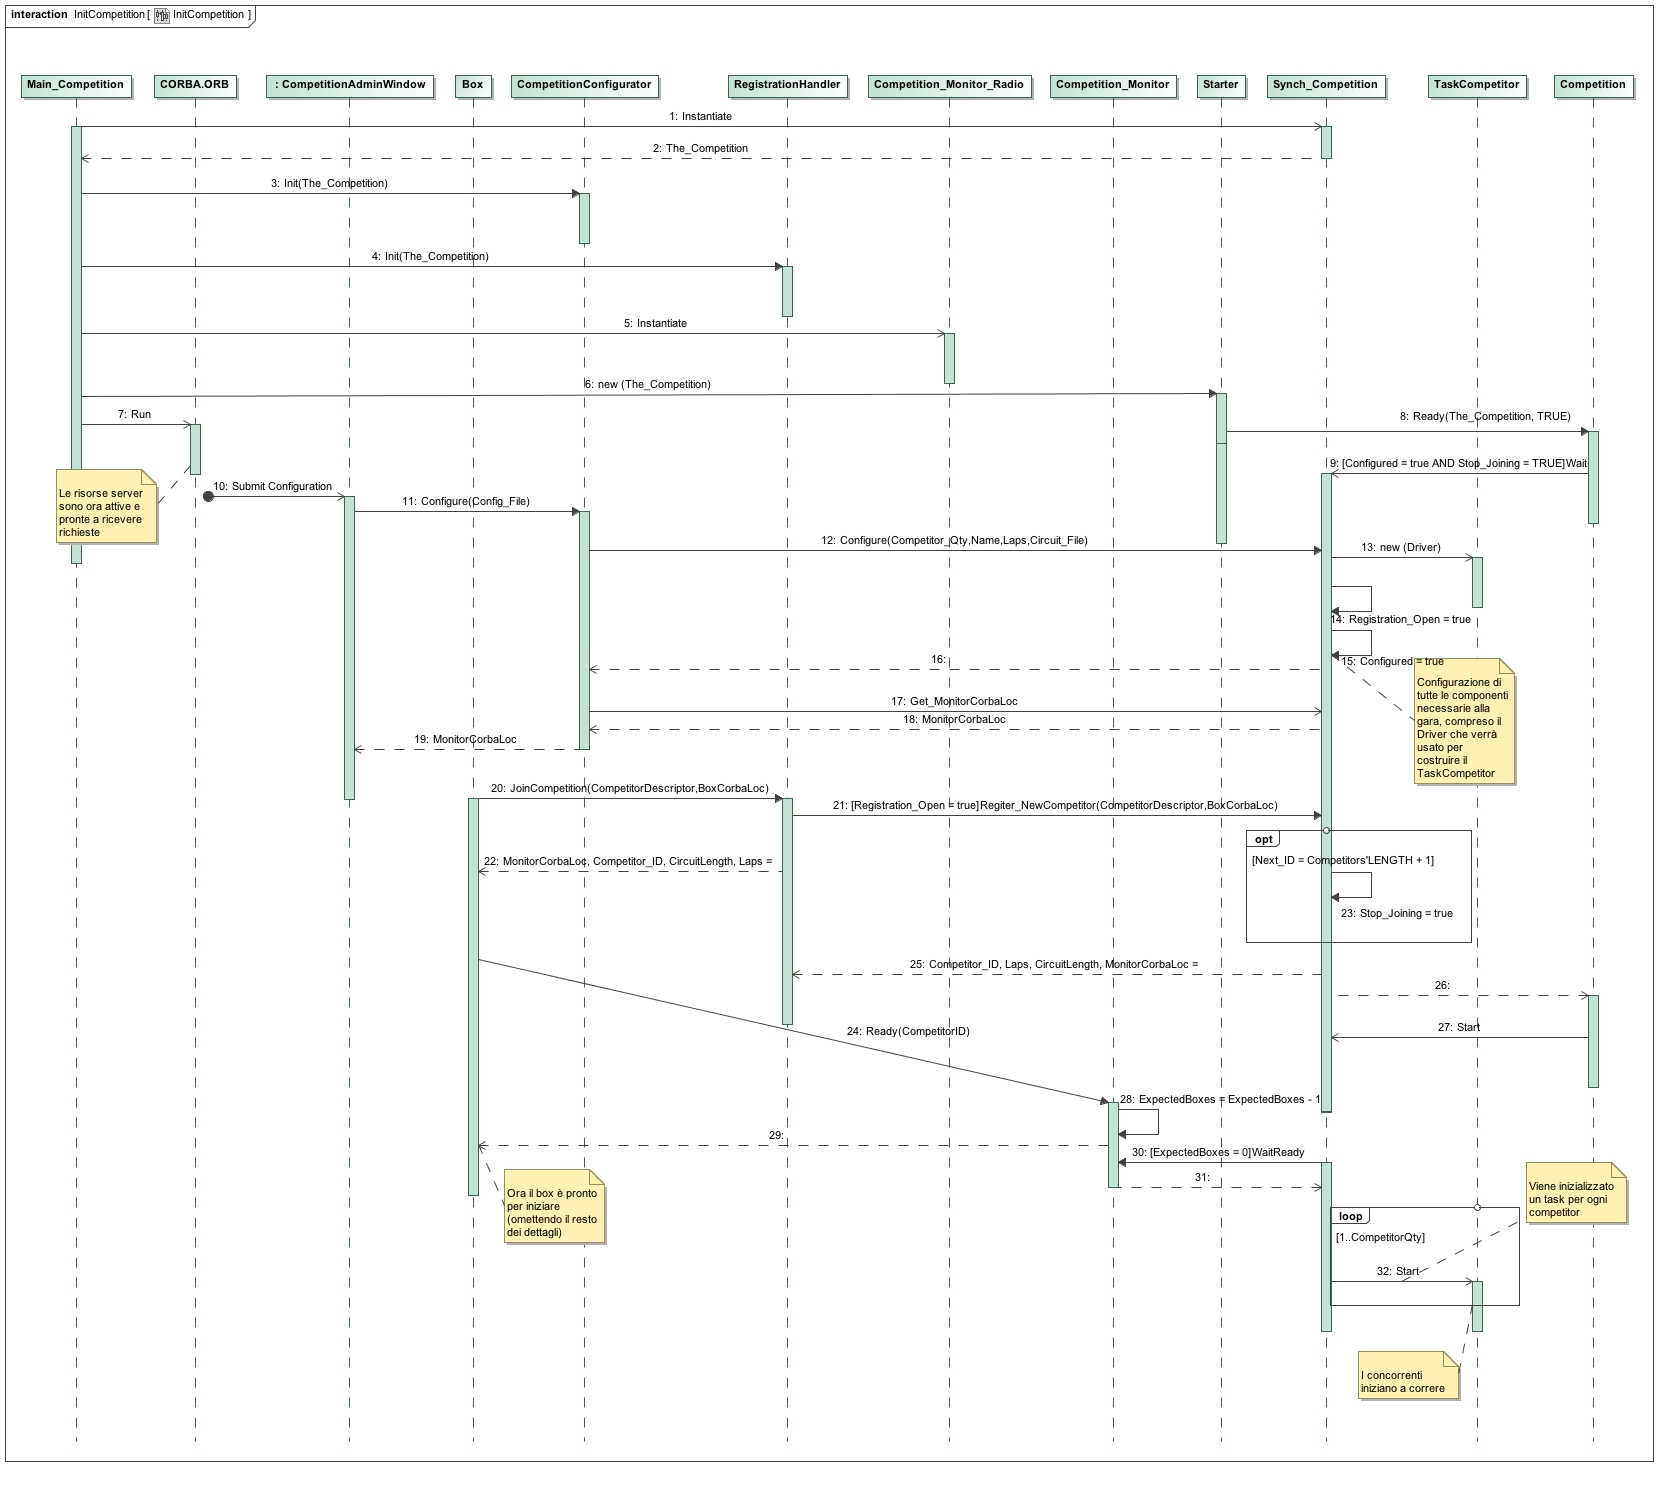
\includegraphics[angle=90,scale=0.35]{img/SequenceDiagrams/InitCompetition.jpg}
\caption{Sequence Diagram - Inizializzazione competizione}
\end{figure}
\end{center}
\clearpage
Una volta avviato il main della competizione, per prima cosa vengono
inizializzati tutti i server, vale a dire \textbf{CompetitionConfigurator},
\textbf{RegistrationHandler} e \textbf{Competition\_Monitor\_Radio}. Viene avviato
un task \textbf{Starter} che rimane in attesa
della configurazione e registrazione concorrenti avvenuti per dare lo
\underline{Start} alla gara. Viene inoltre allocata una risorsa protetta di tipo
\textbf{Synch\_Competition} pensata
per agevolare la fase di init. Ne viene condivisa un'istanza fra
\textbf{CompetitionConfigurator}, \textbf{RegistrationHandler} e
\textbf{Starter}.
Tale risorsa permette di regolare i vari step dell'inizializzazione. Finch\`{e}
la competizione non viene configurata (dal passo \textbf{10} al passo
\textbf{16}),
non sar\`{a} concesso di registrare concorrenti. Una volta configurata la
competizione, viene aperta la guardia \textsc{Registration\_Open} e il metodo
\underline{Register\_NewCompetitor} potr\`{a} essere invocato (in
\textbf{Synch\_Competition}). L'iscrizione dei concorrenti avviene a partire dai
\emph{Box}.
Nel diagramma l'azione iniziale del \emph{Box} è la \textbf{20}. In realt\`{a},
nel nodo del box, viene prima avviato uno script che esegue il main del box
seguito dal main dell'interfaccia (java) di configurazione del concorrente e del
box. A configurazione avvenuta, i parametri vengono inviati al server della
competizione invocando il metodo del server \textbf{Registration\_Handler}
\underline{Join\_Competition}, come scritto nel diagramma. A iscrizione
avvenuta, 
i parametri di configurazione della competizione tornati vengono usati per
inizializzare e avviare il box e relativi task grazie a cui successivamente
sar\`{a} possibile mandare il messaggio di \underline{Ready} alla competizione.
Quando tutti i concorrenti sono stati registrati (\textbf{23}), bisogna rimanere
in attesa della conferma di avvenuta inizializzazione dei \emph{Box}. Ci\`{o}
avviene quando il thread del task \textbf{Starter} invoca il metodo
\underline{Start} del \textbf{Synch\_Competition}, dentro cui viene messo in
attesa
sul \textbf{Competition\_Monitor} tramite \underline{Wait\_Ready}. Quando tutti
i \emph{Box} hanno dato l'ok, significa che sono pronti per ricevere
richieste dai rispettivi competitor e la gara pu\`{o} cominciare. Vengono
cos\`{i} avviati uno ad uno (\textbf{32}) e la competizione ha inizio.
\subsection{Stop competizione}
Lo stop del sistema avviene su 3 livelli: stop dei task, stop delle interfacce
utente e stop dei server. Vediamo in dettaglio:
\begin{description}
\item{\textbf{Stop dei task}}:\\
i task che devono essere fermati sono i \textbf{TaskCompetitor} lato
competizione e i task \textbf{Update\_Retriever} e \textbf{Strategy\_Updater}
lato box.
I primi si fermano in automatico quando le condizioni dell'auto non permettono
di procedere (benzina finita o gomme troppo usurate) oppure a competizione
finita
(fine ultima lap). I secondi due si fermano quando l'aggiornamento fornito dal
monitor della competizione segnala uno stato dell'auto a causa di cui il 
concorrente non pu\`{o} procedere (poca benzina o molta usura gomme), oppure
quando il concorrente finisce l'ultima lap (sempre grazie agli aggiornamenti);
\item{\textbf{Stop delle interfacce utente}}:\\
\`{e} sufficiente chiudere le interfacce con il tasto \textbf{x} in alto a
destra;
\item{\textbf{Stop dei server}}:\\
una volta finita la gara e chiuse le interfacce utente, lo script di avvio
procede l'esecuzione invocando un \textbf{killall -9} sui main avviati,
interrompendo
cos\`{i} anche i task server.
\end{description}
\section{Architettura ad alto livello}
'%%%Architettura alto livello%%%
\subsection{Architettura ad alto livello}
Nella seguente sezione verr\`{a} illustrata l'architettura ad alto livello del sistema sviluppato, 
escludendo i dettagli implementativi e legati al linguaggio.
% Componenti del sistema
\subsubsection{Componenti di sistema}
Le principali componenti del sistema sono:
\begin{description}
\item{Competition}
La \emph{Competition} \`{e} l'unit\`{a} atta ad orchestrare l'avvio e la conclusione della corsa. Tale componente, dunque, \`{e} stata concepita per 
offrire le seguenti funzionalit\`{a}:
\begin{itemize}
\item Configurazione parametri di gara:
	\begin{itemize}
		\item numero di giri;
		\item numero di concorrenti;
		\item circuito;
	\end{itemize}
\item Gestione della sessione di iscrizione e accettazione concorrenti (configurati a livello della componente \emph{Box})
\item Avvio delle componenti necessarie al monitoraggio della gara (quali ad esempio \emph{Monitor})
\item Avvio controllato della competizione vera e propria nel momento in cui tutti i prerequisiti di inizio sono soddisfatti, ovvero:
\begin{itemize}
\item la competizione \`{e} stata configurata correttamente;
\item le componenti di controllo e gestione della competizione sono attive e in attesa di comandi;
\item i concorrenti sono stati correttamente registrati alla competizione e in attesa di partire;
\end{itemize}
\end{itemize}
\item{Competitor}
Il \emph{Competitor} \`{e} l'entit\`{a} pensata ad svolgere la gara. \`{E} caratterizzato dalle seguenti sotto-componenti:
\begin{itemize}
\item \textbf{Auto}, ovvero tutte le caratteristiche fisiche legate all'auto, ovvero:
	\begin{itemize}
		\item motore;
		\item capacit\`{a} del serbatoio;
		\item massima accelerazione;
		\item massima velocit\`{a};
		\item gomme montate (mescola, modello, tipo);
		\item livello usura gomme;
		\item livello della benzina nel serbatoio;
	\end{itemize}
\item \textbf{Guidatore}, cio\`{e} le informazioni che descrivono pi\`{u} dettagliatamente il concorrente in gara:
	\begin{itemize}
		\item nome e cognome pilota;
		\item nome scuderia
	\end{itemize}
\item \textbf{Strategia}, ovvero la strategia che sta adottando il pilota, suggerita dai box e dinamica nel corso della gara:
	\begin{itemize}
		\item style di guida, variabile tra conservativo, normale, aggressivo, a seconda dello stato della macchina e delle
			previsioni fatte dai box
		\item numero di lap prima del pit stop
		\item addizionalmente, quando viene fatto un pit stop, la strategia determina anche quali siano le nuove gomme da montare,
		 	la quantit\`{a} di benzina da avere nel serbatoio e il tempo impiegato per il pit stop.
	\end{itemize}
\end{itemize}
Tutte queste informazioni insieme creano quello che viene definito il concorrente di gara. 
Tali informazioni verranno poi usate nel corso della gara per:
	\begin{itemize}
		\item scegliere al momento giusto la miglior traiettoria da seguire, in base alla presenza o meno di altri concorrenti
			nelle vicinanze e alla difficolt\`{a} del tratto;
		\item fornire costantemente aggiornamenti sul suo stato (tramite una parte del modulo \emph{Stats}, informando il computer di bordo
			riguardo a:
			\begin{itemize}
				\item livello di usura gomme;
				\item livello di benzina;
				\item checkpoint attraversato con tempo di arrivo;
				\item insieme al checkpoint verranno aggiornate le informazioni relative a settore e lap;
				\item velocit\`{a} massima raggiunta.
			\end{itemize}
		\item contattare ad ogni giro il box per ottenere una strategia aggiornata;
		\item se suggerito dai box, effettuare un pitstop;
		\item ritirarsi dalla gara una volta che le condizione dell'auto non permettano di poter correre ulteriormente;
		\item banalmente, continuare a correre fino alla fine delle lap prestabilite, dopodich\`{e} fermarsi.
	\end{itemize}
\item{Circuit}
Il circuito è una risorsa finalizzata ad offrire il piano su cui svolgere la competizione. \`{E} condivisa fra tutti i concorrenti in gara e
offre un insieme di funzionalità per poter conoscere le caratteristiche dei vari tratti della pista (compresi i concorrenti presenti
al momento dell'attraversamento). \`{E} composto dalle seguenti sottocomponenti:
\begin{itemize}
\item \textbf{Checkpoint}
\item \textbf{Path}
\item \textbf{}
\end{itemize}
\item{Stats}
\item{Box}
\item{Radio}
\item{Monitor}
\end{description}
 - lista delle componenti con descrizione ad alto livello del loro scopo
 - se necessario fornire un diagramma delle componenti
% Interazione fra le componenti
\subsubsection{Interazione fra le componenti}
 - descrivere ad alto livello l'interazione fra componenti e se necessario aiutarsi con OCR cards
% Strategia adottata per la correttezza temporale
\subsubsection{Strategia adottata per la correttezza temporale}
% Dimostrazione dell'assenza di stallo
\subsubsection{Assenza di stallo}
%%% Architettura in dettaglio %%
\subsection{Architettura in dettaglio}
% Elenco dei task con descrizione
\subsubsection{Risorse attive}
% Elenco risorse condivise con descrizione
\subsubsection{Risorse passive}
\begin{itemize}
\item{Risorse protette}
\item{Altre risorse}
\end{itemize}
%"Analisi della concorrenza"
\subsubsection{Analisi della concorrenza}
	%. analisi dell'interazione risorse e task (senza menzionare la distribuzione)
	%. dimostrazione assenza di racecondition
	%. dimostrazione assenza di starvation
\begin{itemize}
\item{Interazione tra risorse condivise e task}
\item{Assenza di racecondition}
\item{Assenza di starvation}
\end{itemize}
%"Distribuzione"
\subsubsection{Distribuzione}
	%. Elenco risorse distribuite
	%. Interazione risorse distribuite
	%. Misure di fault tolerance
\begin{itemize}
\item{Componenti distribuite}%Con motivazione
\item{Interazione fra le componenti distribuite}
\item{Misure di fault tolerance}
\end{itemize}
% Inizializzazione gara
\subsection{Inizializzazione competizione}
% Stop gara
\subsection{Stop competizione}

%\section{Competizione}
%\section{Circuito}
%\section{Pista}
%\section{Box}
%\section{Tratto}
%\section{Traiettoria}
%\section{Concorrente}
%\section{Sistema di controllo}
%\section{Interfaccia di monitoraggio}
\section{Analisi del supporto tecnologico}
% Scelta dei linguaggi 
	% Ada 
	% Java
	% Bash per l'avvio
% Scelta tecnologiche per la distribuzione
% Scelta del middleware

%\chapter{Bibliografia}
\appendix
\section{Glossario}
\begin{list}{}
\item \textbf{A}\\
\textsc{Antenna}: a receiver put on the toll lane -check-in -check-out that read the the information of a toll tag to recognize a customer and notify the lane controller of his arrival.\\
\item \textbf{B}\\
\textsc{Bank}: a generic bank that represents the entity intended to handle the toll lane customers' account when the toll lane system perform a transaction.\\
\textsc{Barrier}: a physical obstacle positioned on each check-in and check-out. It is intended to prevent an unauthorized customer to pass through.\\
\item \textbf{C}\\
\textsc{Concorrente}: l'entità costituita da pilota e auto che partecipa alla gara correndo sul circuito.\\
\textsc{Cashier (review)}: employee who works in every toll lane station check-in whose task can be summurized in the lsit below:
\begin{itemize}
	\item receive a customer who wants to pass through the toll lane;
	\item calculate the price based on the vehicle type;
	\item take right amount the money and eventually register the customer;
\end{itemize}
\textsc{Card reader}: the device used to read the customer's credit card and perform the transaction with a bank.\\
\textsc{Check-in}: the entering point of the toll lane. There are two kind of Check-in:
\begin{itemize}
\item Express, where a customer che pass through using a toll tag;
\item Normal, where a customer has to stop and pay (using cash or credit card) before being able to pass.
\end{itemize}
Each Check-in has a barrier.\\
\textsc{Check-out}: the exit point of the toll lane. there are two kind of Check-out:
\begin{itemize}
\item Express, where a customer can pass through using a toll tag;
\item Normal, where a customer has to stop and has his ticket validated by the ticket reader before being abel to pass.
\end{itemize}
Each Check-out has a barrier.\\
\textsc{Customer}: the client of the toll lane.\\
\item \textbf{D}
\item \textbf{E}
\textsc{Enterprise server}:\\
\item \textbf{F}
\item \textbf{G}
\item \textbf{H}
\item \textbf{I}
\item \textbf{J}
\item \textbf{K}
\item \textbf{L}\\
\textsc{Lane Controller}: a software system conceived to offer a communication bridge between the input interfaces of the system (like the touchscreen, the ticket reader ...) and the other components (like the station server, the printer ...).\\
\item \textbf{M}
\item \textbf{N}
\item \textbf{O}
\item \textbf{P}\\
\textsc{Printer}: a physical device used by check-in employee to print tickets.\\
\item \textbf{Q}
\item \textbf{R}
\item \textbf{S}\\
\textsc{Station Server}: a server offering the following services:
\begin{itemize}
\item register the toll lane system customer's activities (through the communication with lane controller);
\item store the information about the current prices for the toll lane system service;
\item provide the enterprise server with all the information concerning the toll lane station activities.
\end{itemize}
\item \textbf{T}\\
\textsc{Ticket}: it's sold to the customer at the toll lane station or in a specialised center. It gives the customer the possibility to use the toll lane. It's used at the check-out to leave the toll lane.\\
\textsc{Ticket reader}: physical device used to recognize a valid ticket and eventually notify the lane controller.\\
\textsc{Toll tag}: a device with an RFID chip used by the customer to pass through the express check-in (and check-out) once readed by the antenna.\\
\textsc{Touchscreen}: the physical interface used by the cashier to execute his activities.\\
\item \textbf{U}
\item \textbf{V}
\item \textbf{X}
\item \textbf{Y}
\item \textbf{W}
\item \textbf{Z}
\end{list}

\section{Manuale utente}
\subsection{Prerequisiti}
Il programma pu\`{o} essere eseguito solo su macchine Unix-like. Inoltre, per la compilazione,
\`{e} necessario disporre delle seguenti componenti:
\begin{itemize}
\item gnatmake 4.4.3
\item gcc 4.4.3
\item librerie \textbf{XmlAda 3.2w} installate con comando \underline{xmlada-config} eseguibile anche senza privilegi di root.\\
In caso contrario, scaricare il pacchetto XMLAda da\\
\url{http://libre.adacore.com/libre/download2/}\\
e, dopo la decompressione, seguire le istruzioni incluse per la compilazione ed installazione.
\item librerie \textbf{PolyORB GPL 2009-20090519 (rev. 144248)} installate con comando \underline{polyorb-config} eseguibile anche 
senza privilegi di root\\
In caso contrario, scaricare il pacchetto PolyORB da\\
\url{http://libre.adacore.com/libre/download2/}\\
e, dopo la decompressione, seguire le istruzioni incluse per la compilazione ed installazione.
\end{itemize}
La versione indicata delle librerie \`{e} quella usata per i test. Non si esclude tuttavia che il programma possa funzionare anche con versioni
appena precedenti o successive.
\subsection{Installazione}
Dalla directory radice, eseguire i seguenti comandi:
\begin{itemize}
\item \emph{make competition}\\
per compilare la componente destinata a ospitare la competizione
\item \emph{make box}\\
per compilare la componente destinata a eseguire il box
\item \emph{make tv}
per compilare la componente che verr\`{a} usata per la TV
\end{itemize}
Le tre componenti hanno make diversi perch\`{e} possono essere compilate ed eseguite su macchine separate, comunicando remotamente.
\subsection{Avvio}
Come per la compilazione, dalla directory radice eseguire il comando desiderato fra i seguenti:
\begin{itemize}
\item \emph{./start\_competition.sh}\\
avvier\`{a} la competizione. Apparir\`{a} il pannello di configurazione (del quale verranno forniti dettagli in seguito)
\item \emph{./start\_box.sh n}\\
avvier\`{a} un numero n box. Per eseguire un test in locale \`{e} possibile avviare tanti box quanti quelli stabiliti durante la configurazione
della competizione. In tal caso, l'interfaccia di configurazione dei box presenter\`{a} nello spazio riservato al corbaloc per la connessione
alla competizione, il corbaloc della competizione caricato dal contesto locale. Se invece si volessero avviare i box in altri nodi, il corbaloc
per la registrazione pu\`{o} essere trovato in \\
\emph{competition\_registrationhandler\_corbaLoc.txt}\\
a competi<ione configurata. 
\item \emph{./start\_tv.sh}\\
inizializza una tv. Anche in questo caso, se il corbaloc della competizione \`{e} presente in locale, verr\`{a} impostato di default nel textbox
dedicato. \`{E} comunque possibile reimpostarlo utilizzando il corbaloc salvato nel file\\
\emph{competition\_monitor\_corbaLoc.txt}\\
a competizione configurata.
\end{itemize}
L'interfaccia TV \`{e} possibile copiarla senza necessit\`{a} di ricompilazione in tutte le macchine ove la si voglia eseguire. E' sufficiente,
una volta compilata, copiare il file \emph{start\_tv.sh} e la directory \emph{obj/java/GUI} (mantenendo la gerarchia intatta) in un qualunque
nodo distribuito ed eseguire lo starter.
\subsection{Terminazione}
Per terminare il programma (box, competizione o tv che sia) premere il tasto ``x'' in alto a destra sulla finestra.
\subsection{Interfaccia box}
Nella prima schermata che appare si può selezionare un file di configurazione da cui caricare i dati per i concorrenti. Se non si seleziona l'opzione si passa alla seconda schermata dove si possono impostare a mano, partendo dai valori di default. 
I parametri impostabili sono:
\begin{enumerate}
\item Impostare il nome del concorrente
\item Impostare il cognome del concorrente
\item Impostare la scuderia del concorrente
\item Impostare il livello di seriet\`{a} del box (come descritto da \ref{box})
\item Impostare la massima capacit\`{a} del serbatoio
\item Impostare il livello di benzina iniziale
\item Impostare la mescola delle gomme montate (le gomme a mescola morbida si consumano pi\`{u} rapidamente)
\item Impostare lo stile di guida del concorrente 
\item Impostare la massima accelerazione della macchina
\item Impostare la massima velocit\`{a} raggiungibile
\item Inserire il corbaloc che fa riferimento al Registration Hanlder
\item Pulsante per avviare la competizione
\item Pulsante per riportare la gui allo stato iniziale
\end{enumerate}
\begin{center}
\begin{figure}[H]
	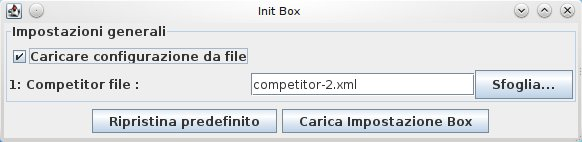
\includegraphics[scale=0.75]{screenshotRelazione/box1.jpeg}
	\caption{Finestra di pre - configurazione del box e del concorrente}
\end{figure}
\end{center}
\begin{center}
\begin{figure}[H]
	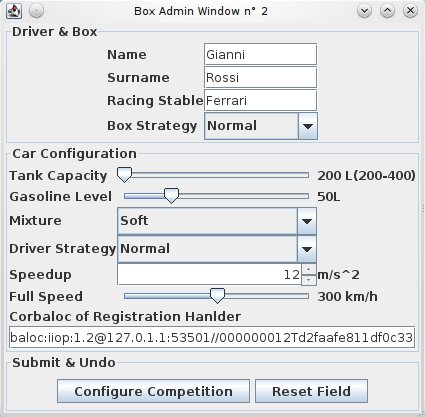
\includegraphics[scale=0.75]{screenshotRelazione/box2.jpeg}
	\caption{Finestra di  configurazione del box e del concorrente}
\end{figure}
\end{center}
Una volta inseriti i dati e premuto il pulsante di avvio della competizione comparir\`{a} una finestra con al suo interno 
\begin{enumerate}
\item Pannello dei consumi medi del concorrente con dati relativi alla benzina (in litri al kilometro) e dell'usura delle gomme (in percentuale relativo a 1 km)
\item Pannello con il log della gara aggiornato a ogni fine settore con dati di tempo di gara, livello di benzina e usura delle gomme
\item Pannello con altre informazioni statiche sulla gara (configurazione iniziale, stile di guida)
\item Pulsante per forzare il pitstop
\end{enumerate}
\begin{center}
\begin{figure}[H]
	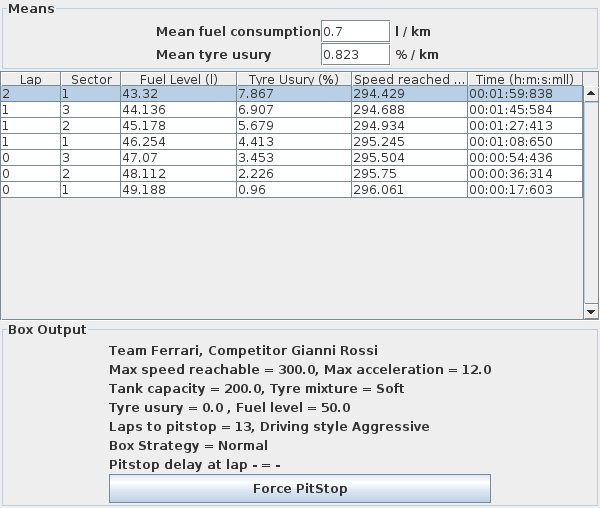
\includegraphics[scale=0.75]{screenshotRelazione/box3.jpeg}
	\caption{Monitor dei box}
\end{figure}
\end{center}
\subsection{Interfaccia competizione}
La prima interfaccia relativa alla competizione serve per impostare la competizione stessa. I parametri da settare sono:
\begin{enumerate}
\item File xml con il tracciato\\
il formato per il file xml del tracciato \`{e} il seguente:
\begin{lstlisting}
<racetrack>
  <sector>
      <checkpoint>
	<length>19.00</length>
	  <mult>7</mult>
	  <angle>140.00</angle>
	  <grip>7.0</grip>
      </checkpoint>
      <!-- altri checkpoint-->
  </sector>
  <!--altri 3 sector strutturati allo stesso modo-->
</racetrack>
\end{lstlisting}
Il checkpoint pu\`{o} avere uno dei seguenti attributi:
\begin{itemize}
\item \textbf{goal=``true''}: obbligatorio in massimo 1 checkpoint. Indica il checkpoint di partenza.
\item \textbf{prebox=``true''}: obbligatorio in massimo 1 checkpoint nel settore 3.
\item \textbf{exitbox=``true''}: obbligatorio in massimo 1 checkpoint nel settore 1.
\end{itemize}
\item Numero di concorrenti richiesti
\item Numero di giri previsti
\item Nome del tracciato
\end{enumerate}
Una volta settati i parameteri e schiacciato il pulsante \emph{Start Competition} verr\`{a} avviato una tv che presenta le informazioni sulle iscrizioni nella parte bassa della finestra. Ogni volta che un concorrente si iscrive compare nella gui e una volta raggiunto il numero di concorrenti stabiliti la gara si avvia e la gui comincia ad offrire i dati disponibili, come spiegato nel paragrafo \ref{interfacciaTv}
\begin{center}
\begin{figure}[H]
	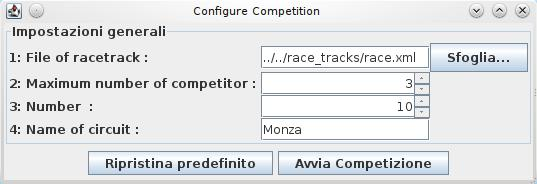
\includegraphics[scale=0.75]{img/ScreenshotRelazione/configureCompetition.jpg}
	\caption{Finestra di configurazione della competizione}
\end{figure}
\end{center}
\subsection{Interfaccia TV}
\label{interfacciaTv}
L'interfaccia della tv consiste in un pannello iniziale con al suo interno un cronometro che scandisce il tempo di aggiornamento delle informazioni seguito da un pannello con le informazioni sul miglior giro e sui migliori tempi nei settori.
L'intervallo per il tempo che scorre \`{e} impostabile se si tratta di una tv configurata tramite il \emph{TvConfigurationWindow}, prestabilito (e molto basso) se si tratta della tv avviata dalla competizione. Il formato della stringa di refresh dev'essere \emph{secondi . millisecondi}.
Questo tempo che scorre \`{e} tempo relativo alla competizione e quindi solidale con il resto del sistema.
Il pannello centrale offre la visualizzazione di due tabelle. La tabella a destra si riferisce all'ultima classifica disponibile mentre a sinistra viene visualizzata la classifica del giro precedente (escluso al primo giro di gara dove viene presentata una tabella vuota).
Nella parte bassa della finestra viene presentato un log della competizione rappresentando a ogni istante di tempo posizione nella pista, numero di checkpoint, numero di settore e giro per ogni concorrente.
\begin{center}
\begin{figure}[h]
	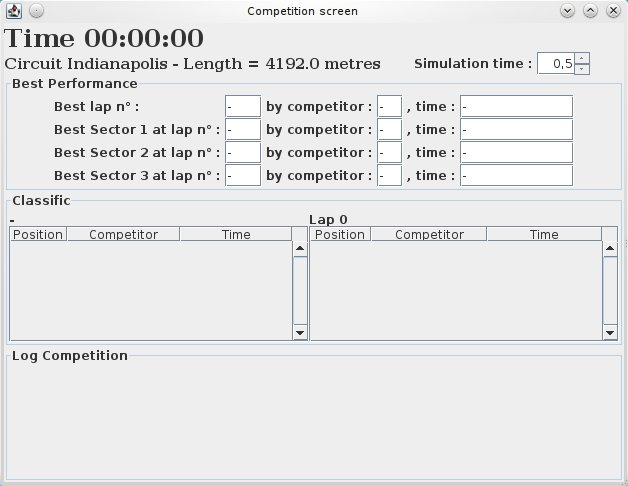
\includegraphics[scale=0.75]{screenshotRelazione/competition2.jpeg}
	\caption{Finestra di visualizzazione dell'andamento della gara}
\end{figure}
\end{center}
\begin{center}
\begin{figure}[h]
	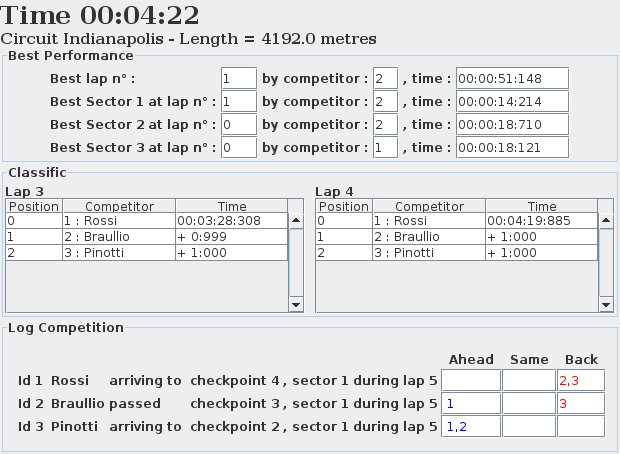
\includegraphics[scale=0.75]{screenshotRelazione/tv2.jpeg}
	\caption{Finestra di visualizzazione dell'andamento della gara - durante la simulazione}
\end{figure}
\end{center}
La componente di avvio dell'interfaccia TV pu\`{o} essere l'interfaccia di competizione oppure una schermata di configurazione dove va inserito il corbaloc del Monitor della competizione e impostato il tempo di refresh per il reperimento delle informazioni. Il pulsante (presente solo nel monitor della competizione) presente in alto a destra permette di modificare il tempo della simulazione.
Nel pannello con il log della competizione sono presenti tre campi per ogni concorrente che rappresentano rispettivamente i concorrenti davanti a lui, nello stesso tratto e dopo di lui.
\begin{center}
\begin{figure}[H]
	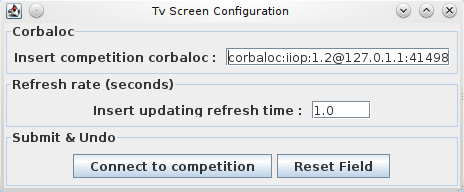
\includegraphics[scale=0.75]{img/ScreenshotRelazione/configurationScreen.jpg}
	\caption{Finestra di configurazione della tv}
\end{figure}
\end{center}

\end{document}
